\chapter{Introducción}
\section{Definición del problema}   
La metrología monocular, es decir, a partir de una única imagen, conocida como \emph{Single View Metrology} (SVM) en inglés, se 
refiere a la estimación de propiedades métricas del mundo tridimensional a partir de una sola vista bidimensional~\cite{VisionBookMIT,Hartley2004}. 
Este enfoque es especialmente útil en situaciones donde no es posible o práctico capturar múltiples imágenes desde diferentes ángulos, ya 
sea por limitaciones físicas, temporales o logísticas. El interés en este campo ha crecido en paralelo con los avances en visión 
por computador, aprendizaje profundo y la disponibilidad de grandes conjuntos de datos. Desde sus orígenes, técnicas 
como las presentadas por~\cite{CriminisiApplications, CriminisiReconstruction, CriminisiPaintings} han demostrado que es posible 
inferir medidas reales si se cuenta con ciertos supuestos geométricos, como líneas paralelas, puntos de fuga o planos rectangulares.
\par
Sin embargo, la aplicación de SVM en entornos naturales o no controlados, conocida como \emph{Single View Metrology in the Wild}~\cite{SVMIW}, 
plantea una serie de dificultades. En primer lugar, los métodos clásicos dependen fuertemente de la existencia de 
estructuras geométricas visibles y bien definidas~\cite{VisionBookMIT}, lo que limita su aplicabilidad a imágenes reales 
donde estas condiciones raramente se cumplen. Además, factores como la iluminación variable, la distorsión por lente, la oclusión, 
la falta de información de calibración de cámara, y la diversidad de escalas y perspectivas complican aún más la estimación precisa 
de medidas métricas~\cite{VisionBookMIT}, véase la Figura~\ref{fig:PerspectiveIlusion}.

\begin{figure}[!ht]
\begin{center}
    \subfloat{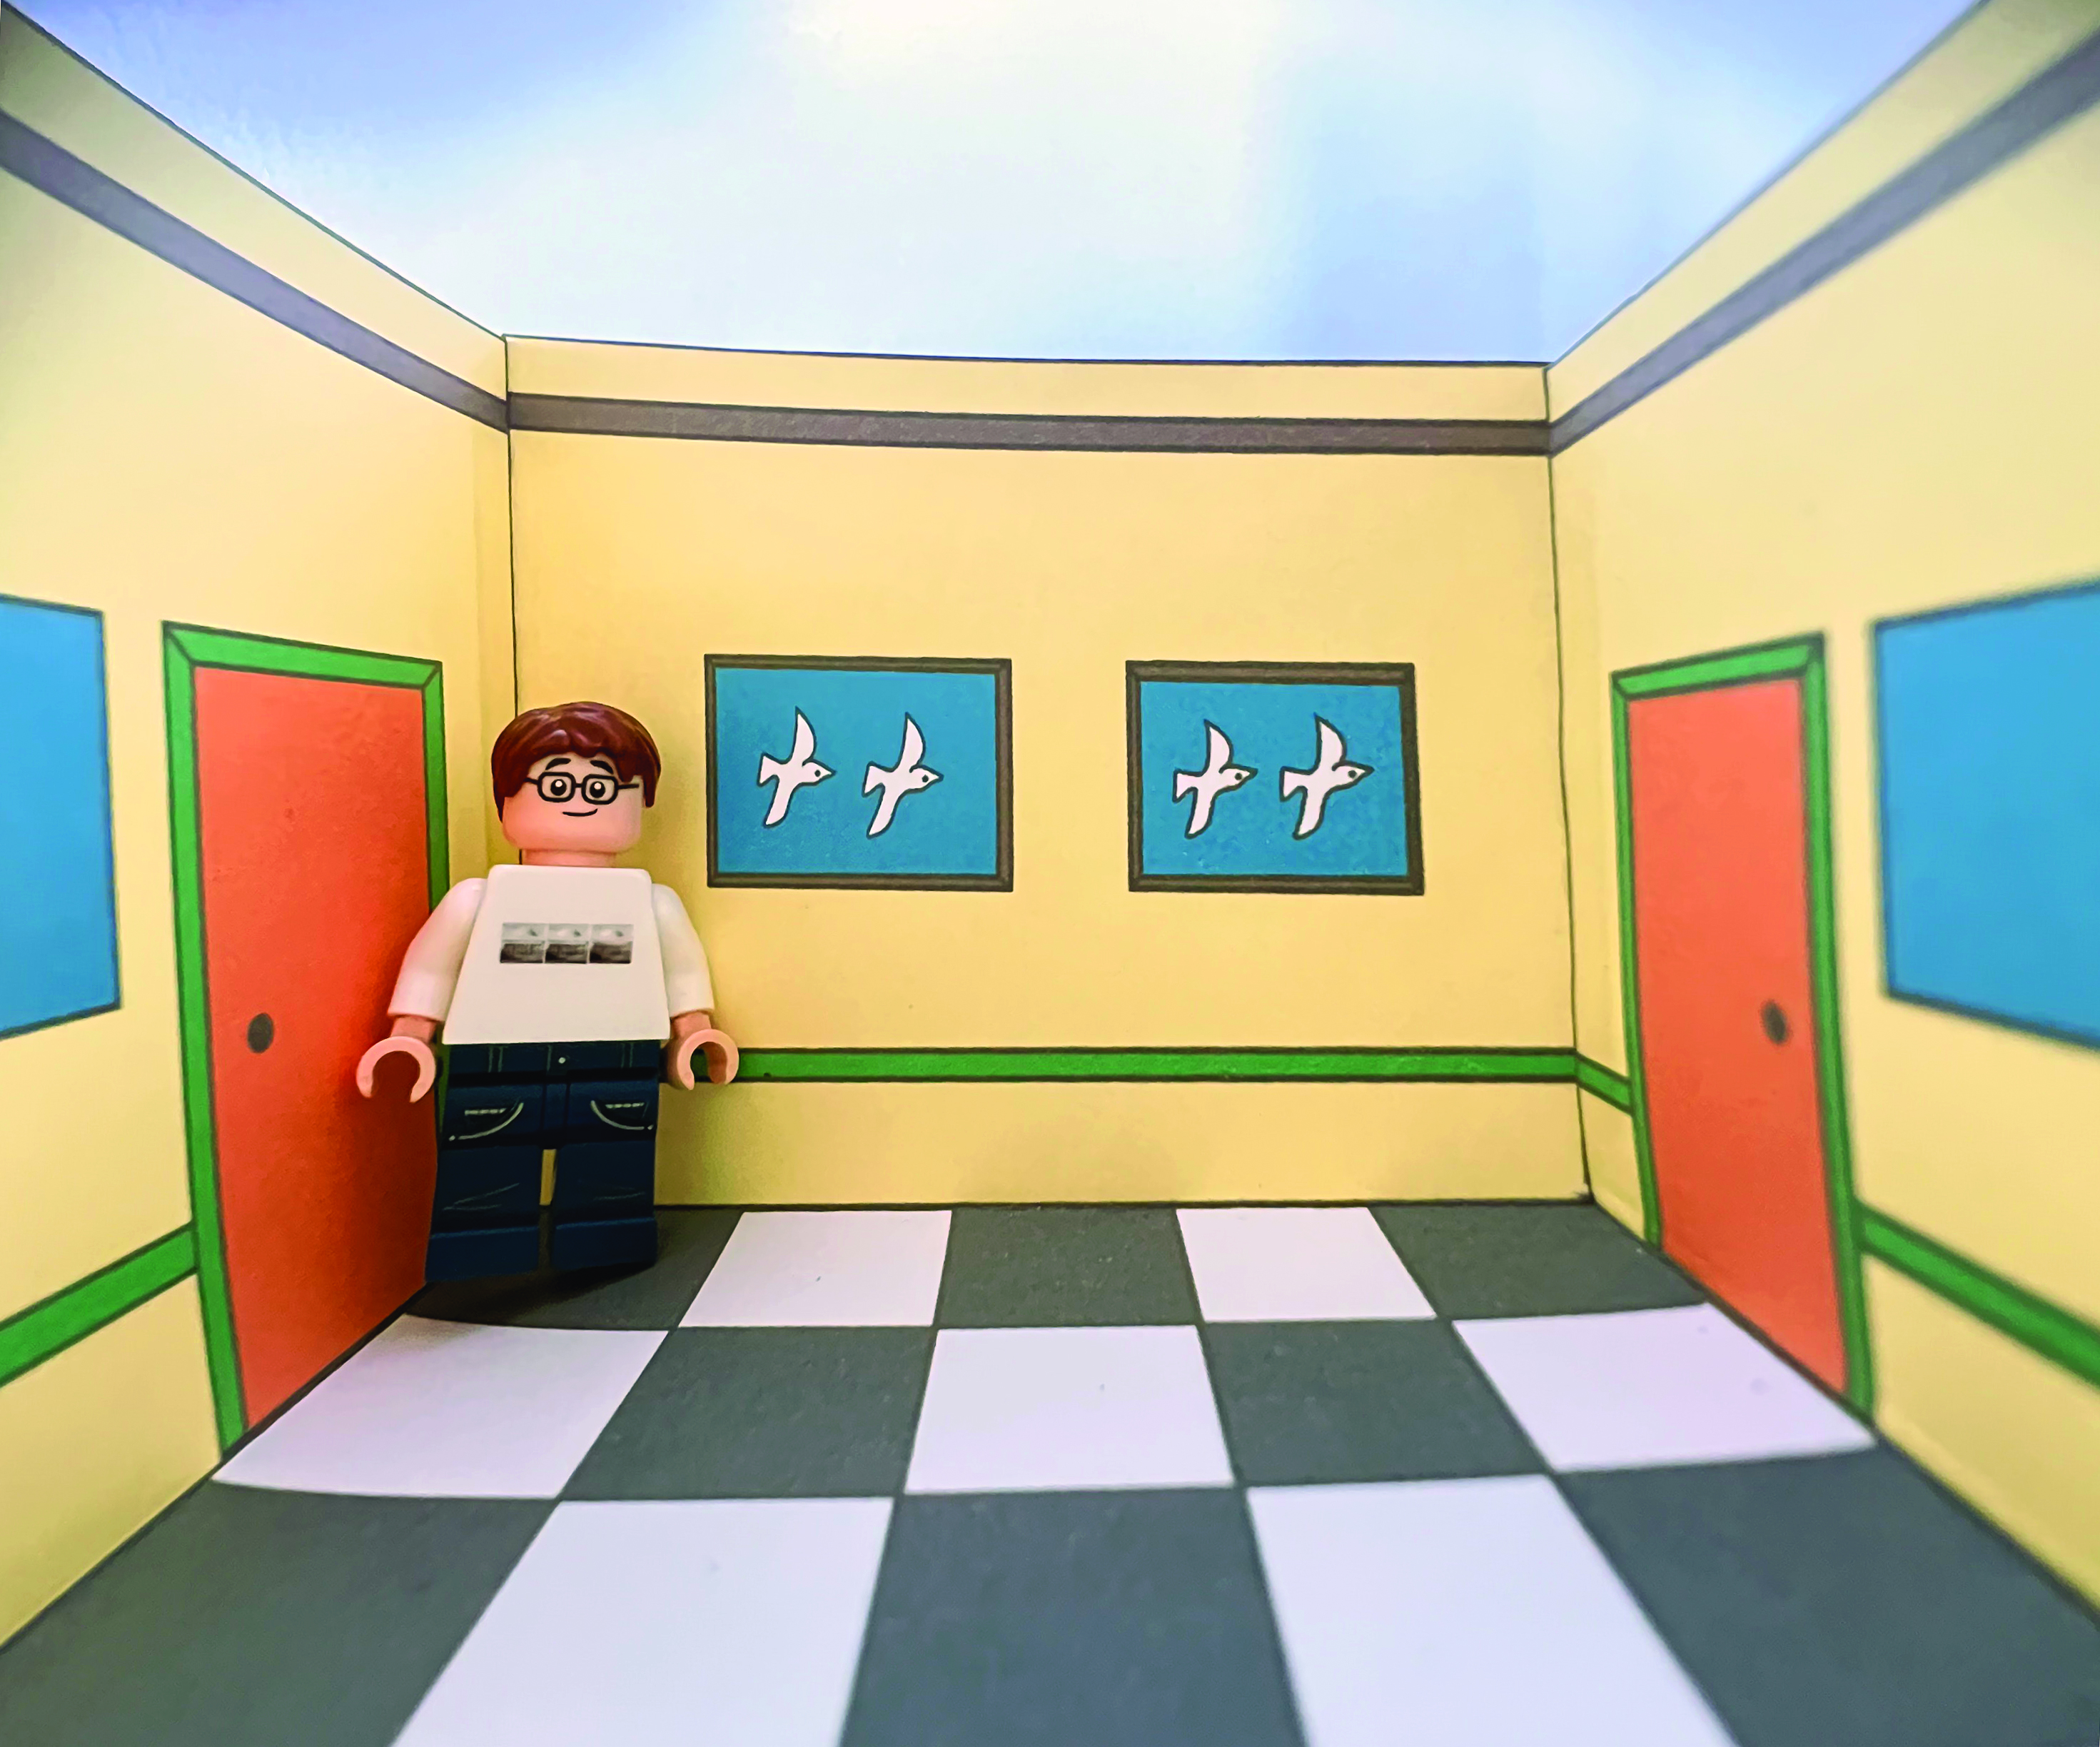
\includegraphics[width=0.325\textwidth]{imagenes/chapter2/LegoLeftSmall}}
    \subfloat{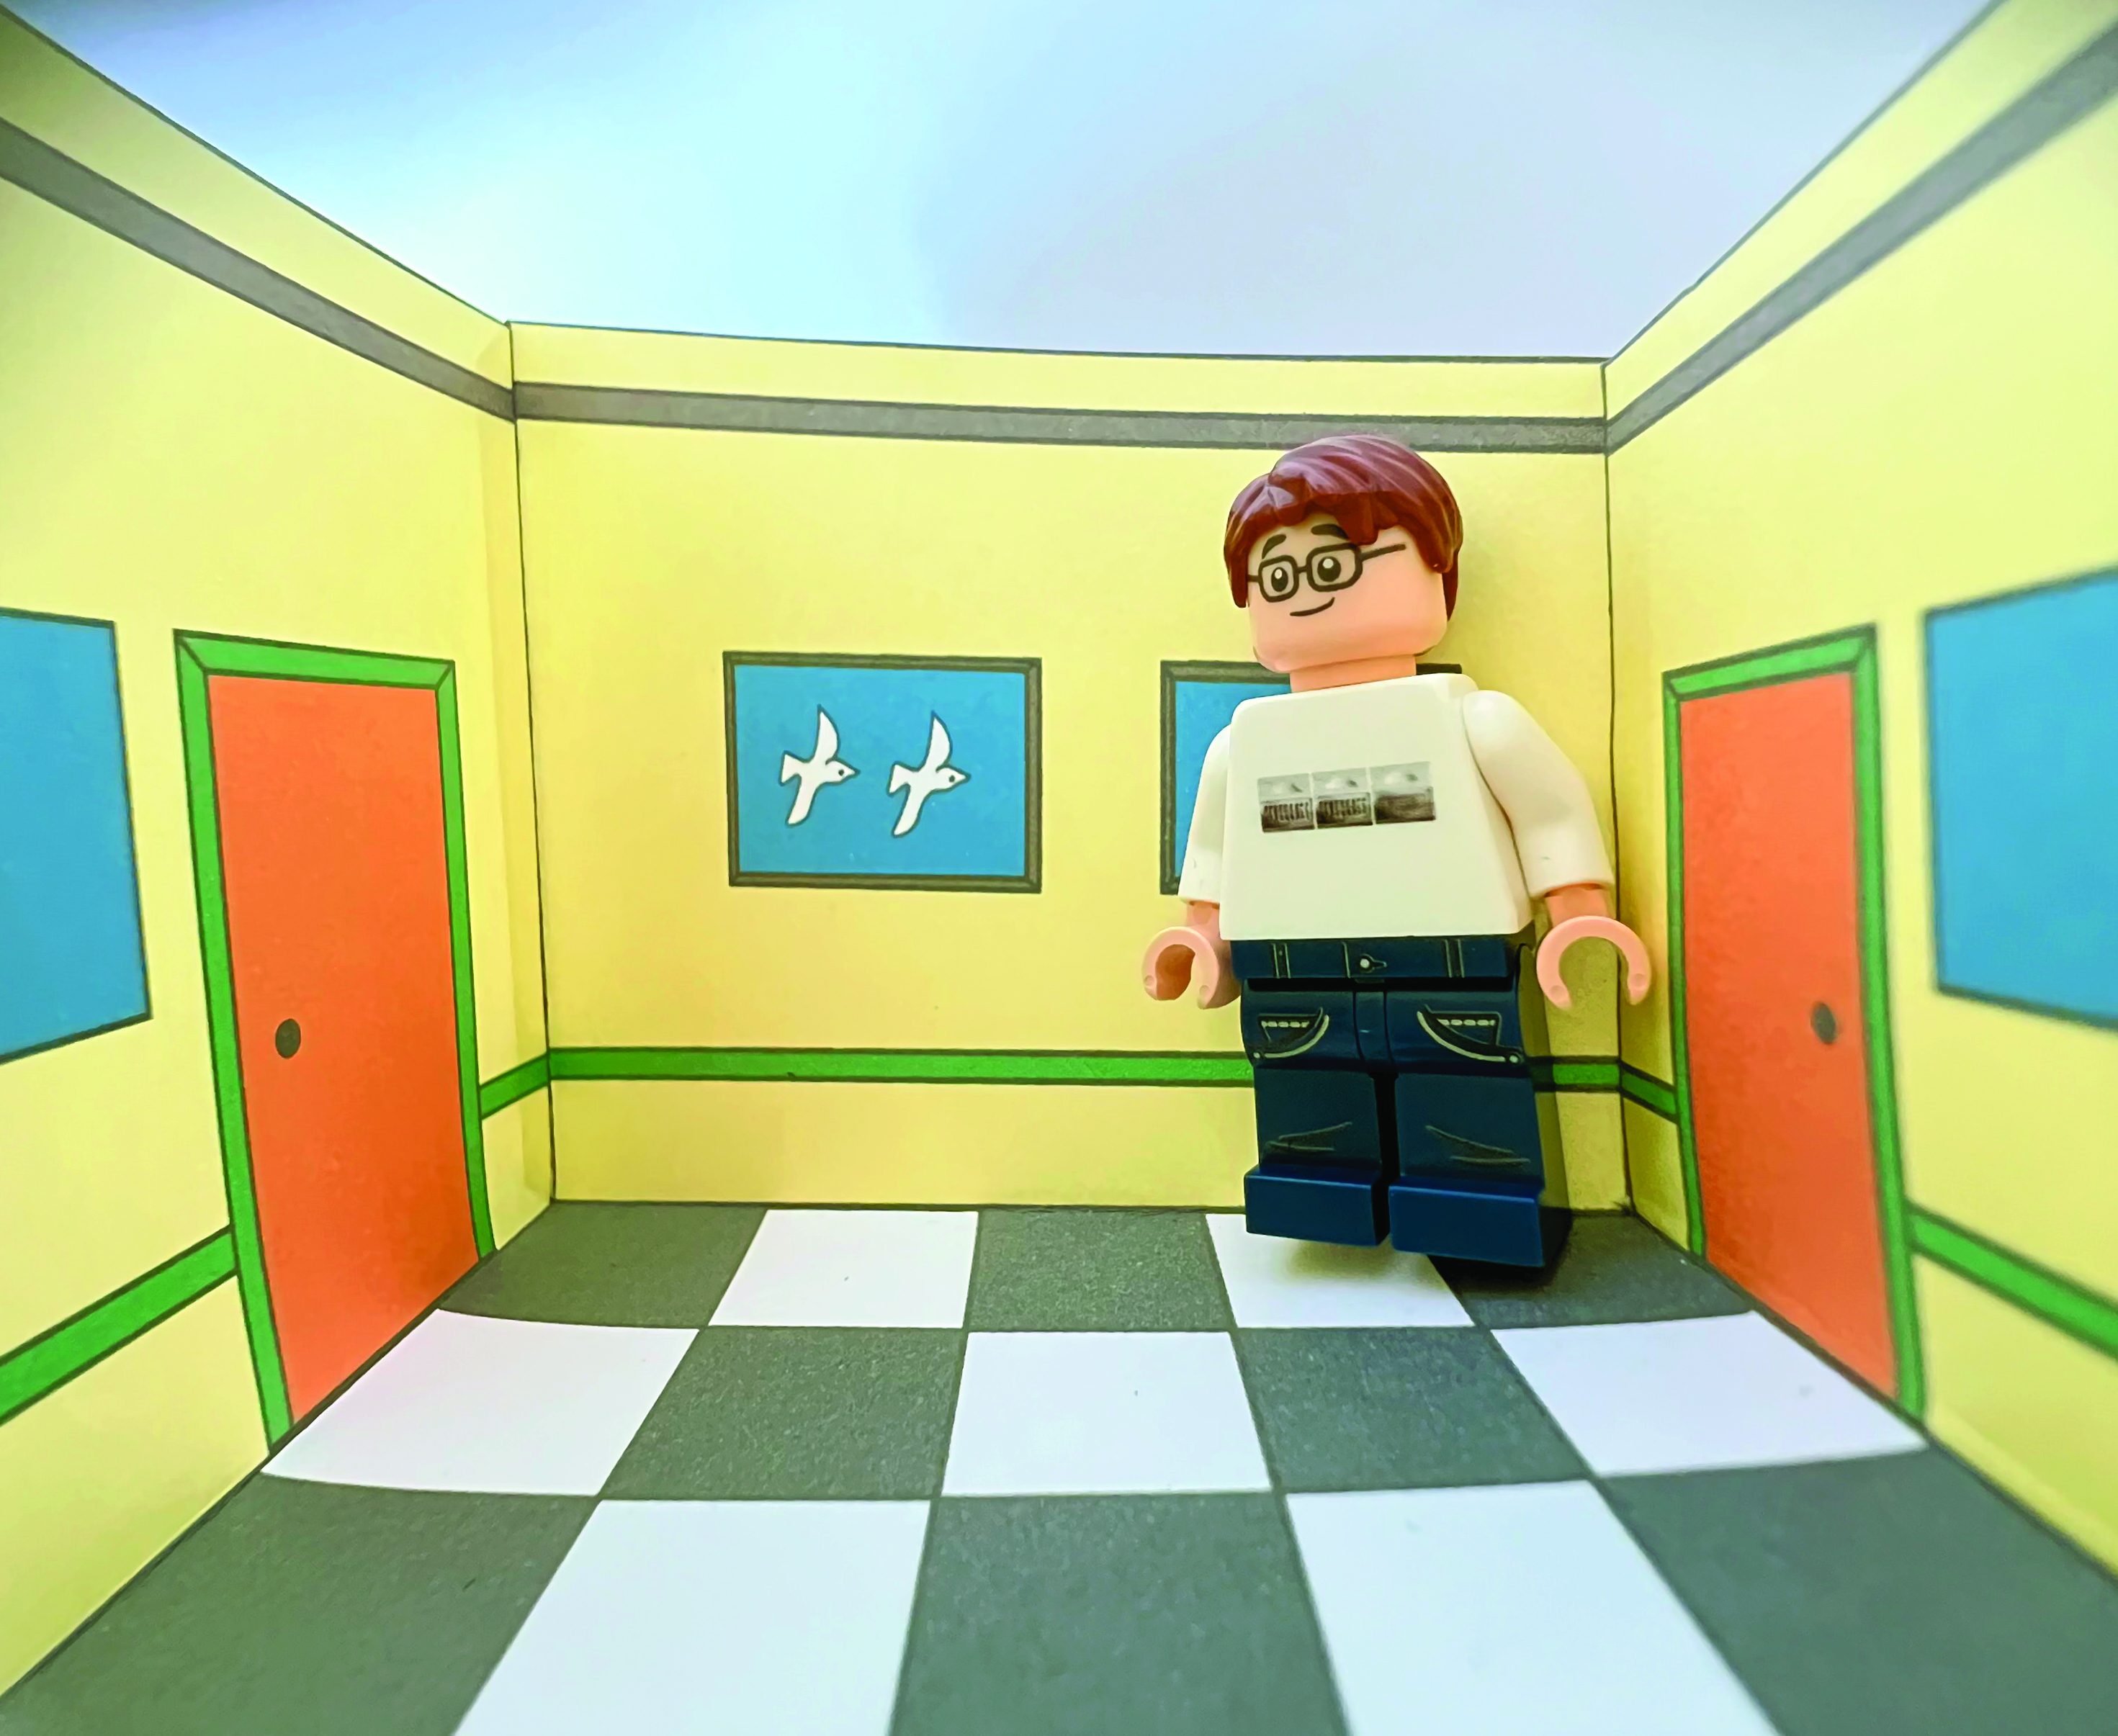
\includegraphics[width=0.33\textwidth]{imagenes/chapter2/LegoRightBig}}
    \subfloat{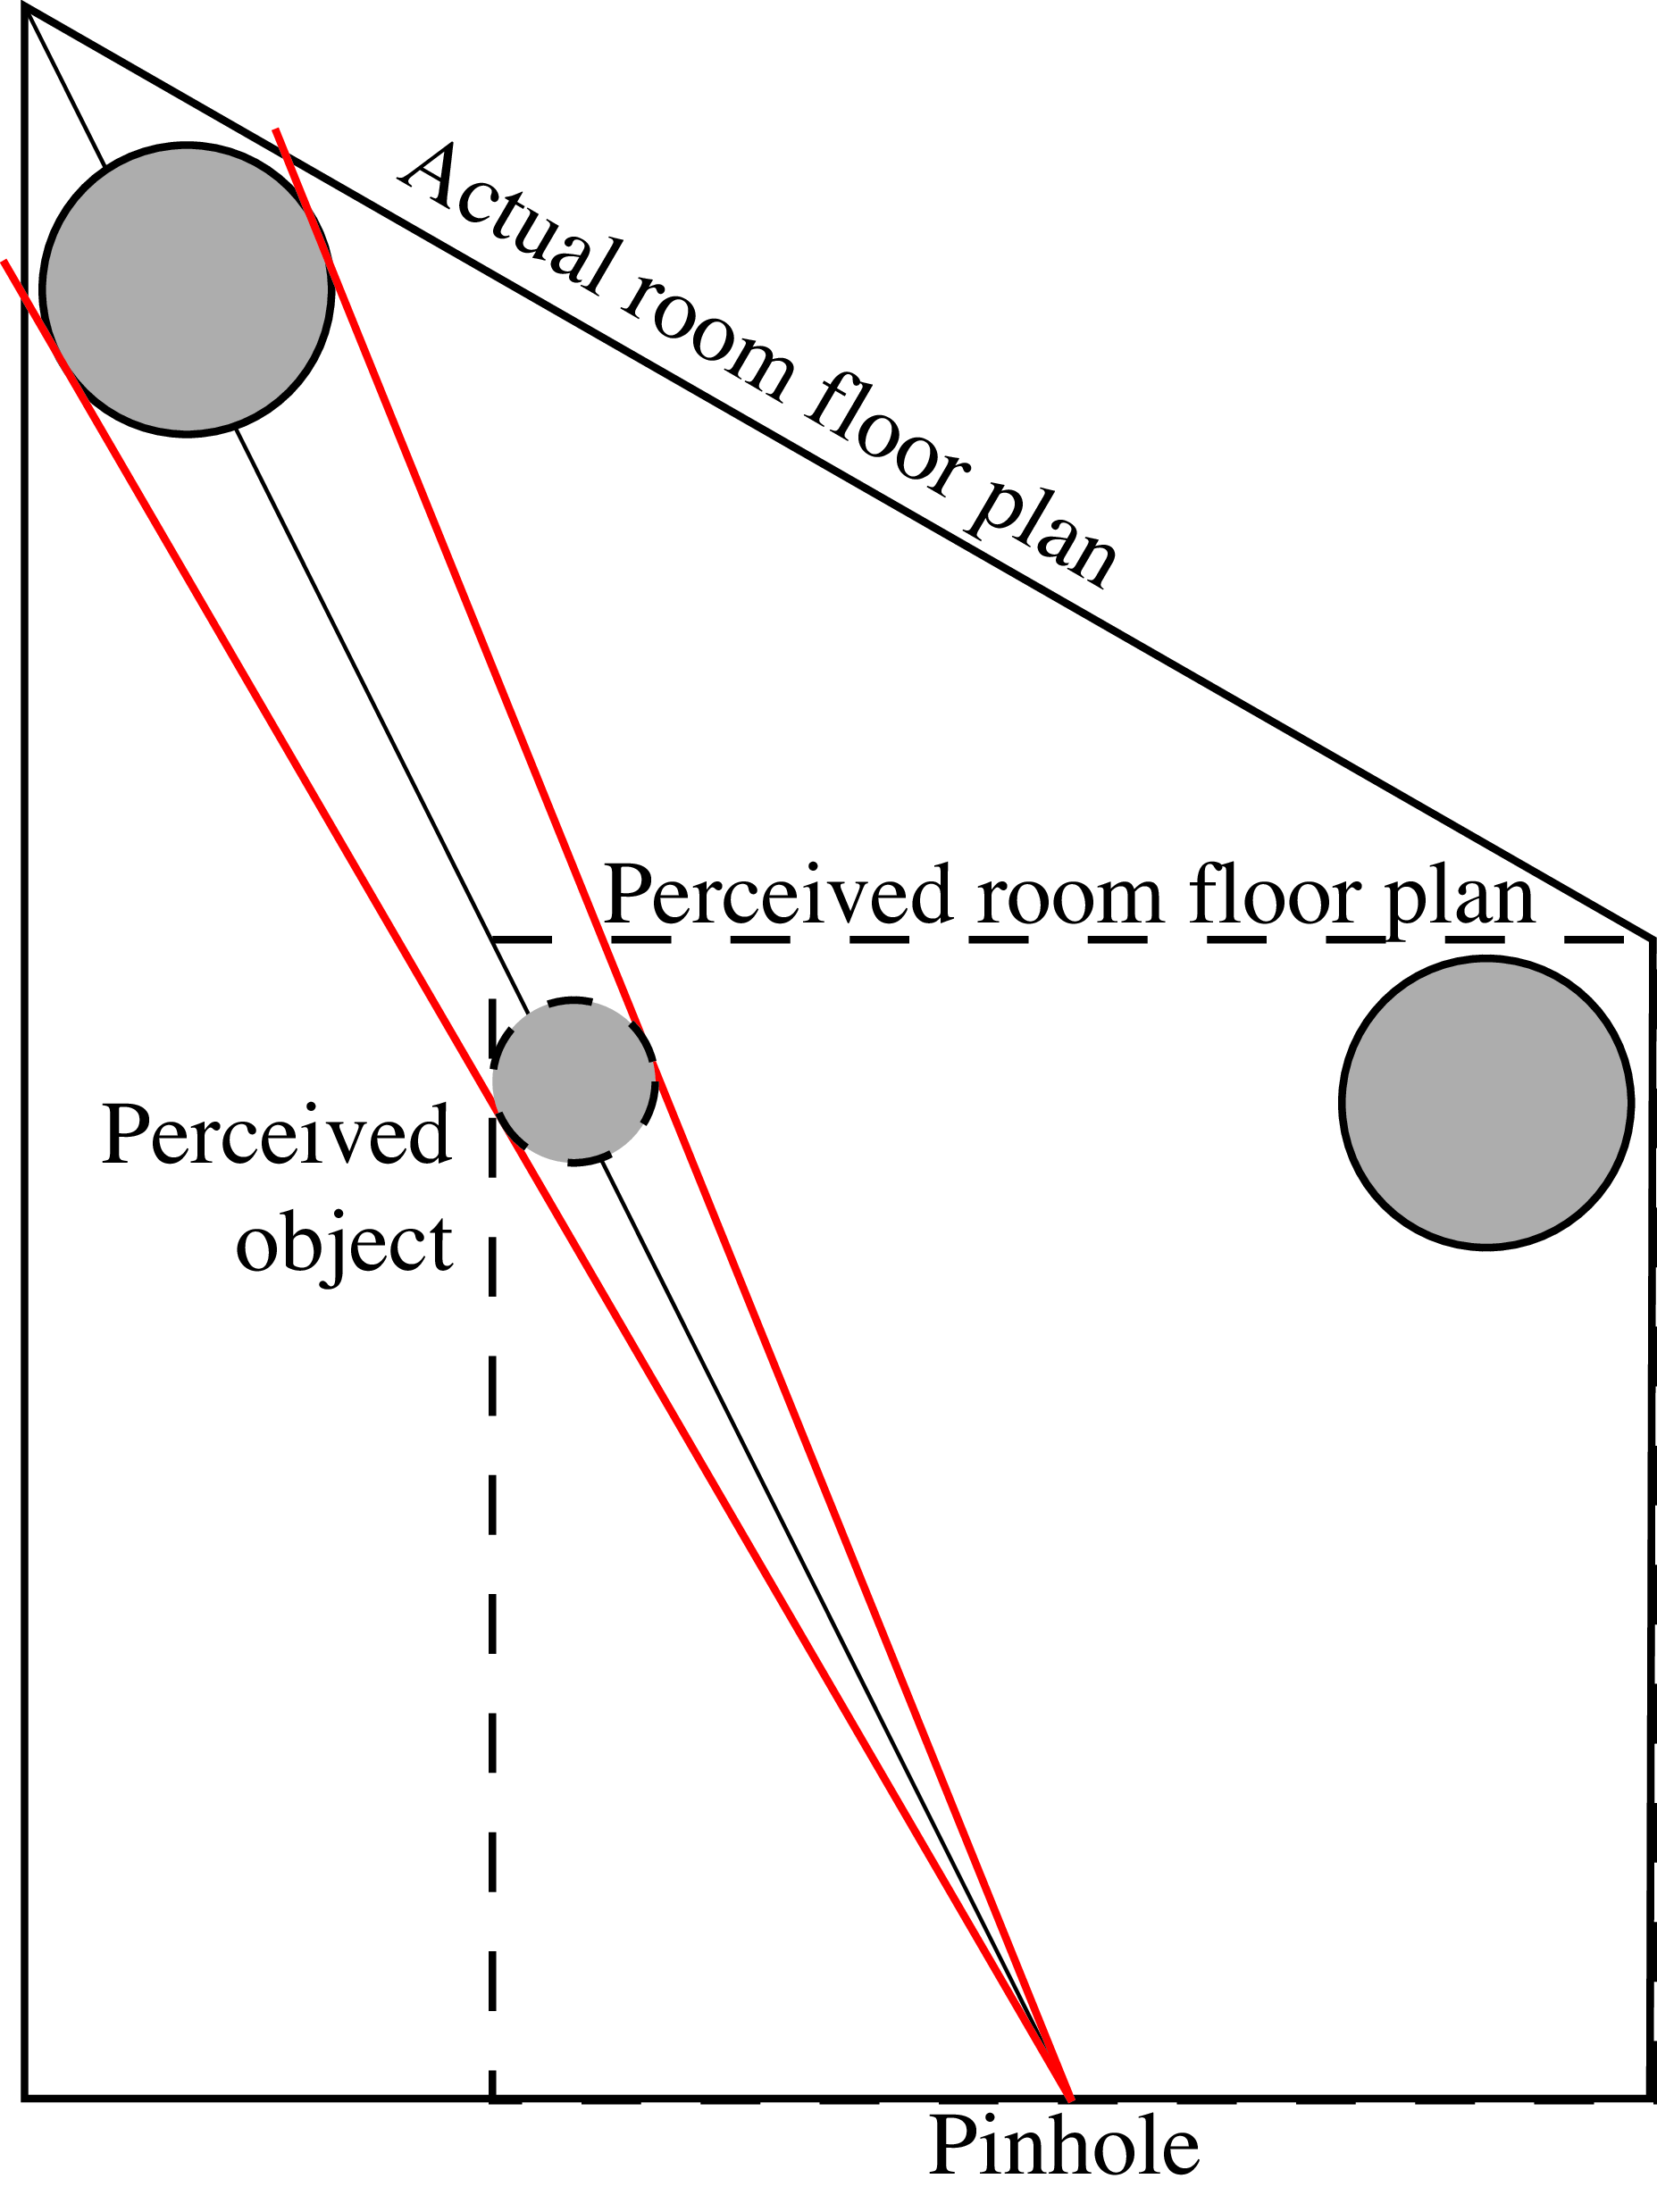
\includegraphics[width=0.2\textwidth]{imagenes/chapter2/AmesRoom}}
\end{center}
\caption{Ilusión óptica que ocasiona a que un mismo objeto, el muñeco de lego, se vea de diferente tamaño según la posición en la habitación
de Ames (menor en la imagen a la izquierda que en la imagen central). La habitación de Ames está construida de forma irregular de forma que al mirar desde un punto en concreto aparenta completamente rectangular, véase la imagen a la derecha.
Ilustraciones sacadas de~\cite{VisionBookMIT}.
}\label{fig:PerspectiveIlusion}
\end{figure}

El auge del aprendizaje profundo ha abierto nuevas oportunidades para abordar estas limitaciones, permitiendo inferir información a 
partir de patrones visuales aprendidos en grandes conjuntos de datos~\cite{PascalVisualObjectChallenge, ImageNet, EffectivenessOfData}. Sin embargo, estas aproximaciones
aún enfrentan desafíos importantes. Uno de ellos es la ambigüedad inherente a la escala absoluta en imágenes monoculares.
Aunque es posible inferir relaciones métricas relativas o proporcionales, sin una referencia explícita o contexto adicional, 
la escala real sigue siendo indeterminada~\cite{DepthFromSingleImage}. Asimismo, la falta de conjuntos de datos etiquetados específicamente para 
tareas de metrología en imágenes reales dificulta la evaluación objetiva del desempeño de estos sistemas~\cite{SVMIW,Metric3Dv2,}.

Dado este panorama, el presente trabajo busca investigar cómo se puede avanzar hacia sistemas robustos de metrología monocular en el mundo real, 
combinando principios geométricos clásicos con técnicas modernas de aprendizaje automático. Progresar en esta línea de investigación 
permitiría construir herramientas prácticas para usuarios sin conocimientos técnicas, como aplicaciones móviles para 
estimación de dimensiones, reconstrucción histórica o inspección visual, democratizando el acceso a capacidades avanzadas 
de visión por computador, con impacto directo a sectores industriales y sociales.
El proyecto esta disponible en \url{https://github.com/briansenas/TFM_SVMIW}.

\section{Motivación}
La metrología es una disciplina fundamental en múltiples ámbitos industriales y científicos, ya que permite realizar mediciones precisas del entorno físico. 
Sin embargo, muchas de las técnicas actuales requieren equipamiento especializado, múltiples vistas o configuraciones controladas del entorno (saber la posición y rotación de la cámara, las características de la misma, la distancia al objeto o más).
En este contexto, la \emph{metrología monocular en entornos no controlados}, se presenta como una alternativa asequible de obtener medidas físicas a partir de una única imagen
sin tener información a priori.
\par
Este campo emergente busca desarrollar métodos robustos y generalizables que funcionen en imágenes capturas en condiciones reales, como pueden ser 
fotografías de redes sociales, grabaciones de seguridad o vídeos deportivos. Esto plantea retos técnicos significativos.
No obstante, la posibilidad de extraer información métrica a partir de imágenes tomadas con cámaras convencionales, sin necesidad de calibración previa o escenas controladas, 
abre la puerta a una amplia gama de aplicaciones reales~\cite{HoiemPopUp,HoiemObjectsInPerspective,CriminisiApplications, CriminisiReconstruction, CriminisiPaintings, SingleViewExerciseQuantification, ObjectsIntoPhotos}. 
\begin{enumerate}
    \item \textbf{Entornos forenses:} Estimación de la estatura de sospechosos o víctimas a partir de grabaciones de cámaras de vigilancia, sin necesidad de intervención pericial directa.
    \item \textbf{Seguridad en espacios públicos:} Sistemas inteligentes capaces de realizar estimaciones biométricas sin infraestructura adicional.
    \item \textbf{Biomecánica en deportes y salud:} Análisis postural o del movimiento en atletas y pacientes sin necesidad de equipamiento especializado, facilitando estudios en el hogar o en entornos no clínicos.
    \item \textbf{Arquitectura y reconstrucción de escenas:} Cálculo de medidas reales de estructuras a partir de imágenes tomadas por usuarios, por ejemplo, para obtener planos aproximados de interiores sin escáneres 3D. Insertar objetos en escenas.
	\item \textbf{Geometría en pinturas:}: Comparación de alturas entre individuos en pinturas o análisis de formas geométricas y patrones.
\end{enumerate}

En el ámbito de la visión por computador se requieren herramientas de metrología más accesibles y confiables. 
En este sentido, contribuir al desarrollo de soluciones que permitan extraer medidas fiables a partir de una sola imagen puede tener un impacto significativo en la democratización de tecnologías de medición, con efectos positivos en ámbitos como la justicia, la salud o la ingeniería.
Por todo ello, se considera que el presente Trabajo Fin de Máster puede suponer una aportación relevante, tanto a nivel teórico como práctico, en el avance de técnicas robustas de metrología monocular aplicadas a contextos reales y no controlados.

\section{Objetivos}
El objetivo principal de este Trabajo Fin de Máster (TFM) es desarrollar 
un \textbf{sistema de estimación automática de la estatura de individuos a partir de una sola imagen}, 
utilizando técnicas de metrología monocular. Los objetivos específicos incluyen:
\begin{enumerate}
    \item Revisar el estado del arte en técnicas de estimación de medidas antropométricas a partir de imágenes.
    \item Implementar y validar un algoritmo basado en principios de metrología visual que estime con precisión la estatura de una persona.
    \item Probar el sistema en diferentes contextos y con variabilidad en las condiciones de iluminación, perspectiva y posición de las personas.
\end{enumerate}
\section{Planificación del proyecto}
Al planificar el proyecto, es fundamental tener en cuenta que el TFM 
tiene una carga de 12 créditos ECTS, donde cada 
crédito representa aproximadamente 25 horas de trabajo. 
En total, se estima que se necesitarán alrededor de 300 horas para llevar a cabo 
el proyecto.  Considerando que el segundo cuatrimestre tiene aproximadamente 20 semanas, 
se requerirá dedicar al TFM unas 15 horas por semana, lo cual equivaldría a unas 3 horas 
diarias durante 5 días a la semana.

Dada la naturaleza del proyecto, cuya complejidad en términos de requisitos y tamaño 
del equipo de trabajo no es elevada, se utilizará un ciclo de vida en cascada~\cite{ModeloEnCascada} con realimentación.
Dicho ciclo de vida se basa en un desarrollo lineal divido en fases, en el cuál antes 
de empezar la siguiente fase se evalúa los resultados obtenidos en la fase anterior. 
De esta forma, se pueden adaptar las fases siguientes a los posibles 
nuevos hallazgos de las fases anteriores.
Las fases del ciclo de vida son: 
\begin{itemize}
  \item Análisis de requisitos: Consiste en reuniones iniciales con los clientes, 
    en este caso los directores del TFM. Se organiza el análisis bibliográfico 
    del problema de metrología monocular, se plantean los objetivos y criterios de aceptación.
  \item Diseño: Consiste en la investigación y selección de métodos conforme 
    al análisis anterior, tanto para la resolución como la validación de la solución. 
    Así como pruebas preliminares y diseño del software de experimentación. 
  \item Implementación: Consiste en la adaptación de las técnicas encontradas, 
      búsqueda de puntos de mejoría y desarrollo del producto mínimo viable. 
  \item Pruebas: Realización de diversos experimentos de validación, 
      comparando desde la metrología con parámetros estimados con una técnica de calibración manual estándar, 
      calibración basada en características de las cámaras y las estimadas por el algoritmo final.
\end{itemize}
\begin{table}[htp]
\centering
\resizebox{\textwidth}{!}{%
\begin{tabular}{|c|c|llll|llll|lllll|llll|llll|}
\hline
\rowcolor[HTML]{FFC702} 
\cellcolor[HTML]{FFC702} & \cellcolor[HTML]{FFC702} & \multicolumn{4}{c|}{\cellcolor[HTML]{FFC702}\textbf{Mayo}} & \multicolumn{4}{c|}{\cellcolor[HTML]{FFC702}\textbf{Junio}} & \multicolumn{5}{c|}{\cellcolor[HTML]{FFC702}\textbf{Julio}} & \multicolumn{4}{c|}{\cellcolor[HTML]{FFC702}\textbf{Agosto}} & \multicolumn{4}{c|}{\cellcolor[HTML]{FFC702}\textbf{Septiembre}} \\ \cline{3-23} 
\rowcolor[HTML]{FFC702} 
\multirow{-2}{*}{\cellcolor[HTML]{FFC702}\textbf{Tarea}} & \multirow{-2}{*}{\cellcolor[HTML]{FFC702}\begin{tabular}[c]{@{}c@{}}\textbf{Semanas -}\\ \textbf{Horas}\end{tabular}} & \multicolumn{1}{c}{\cellcolor[HTML]{FFC702}07} & \multicolumn{1}{c}{\cellcolor[HTML]{FFC702}14} & \multicolumn{1}{c}{\cellcolor[HTML]{FFC702}21} & \multicolumn{1}{c|}{\cellcolor[HTML]{FFC702}28} & \multicolumn{1}{c}{\cellcolor[HTML]{FFC702}04} & \multicolumn{1}{c}{\cellcolor[HTML]{FFC702}11} & \multicolumn{1}{c}{\cellcolor[HTML]{FFC702}18} & \multicolumn{1}{c|}{\cellcolor[HTML]{FFC702}25} & \multicolumn{1}{c}{\cellcolor[HTML]{FFC702}02} & \multicolumn{1}{c}{\cellcolor[HTML]{FFC702}09} & \multicolumn{1}{c}{\cellcolor[HTML]{FFC702}16} & \multicolumn{1}{c}{\cellcolor[HTML]{FFC702}23} & \multicolumn{1}{c|}{\cellcolor[HTML]{FFC702}30} & \multicolumn{1}{c}{\cellcolor[HTML]{FFC702}06} & \multicolumn{1}{c}{\cellcolor[HTML]{FFC702}13} & \multicolumn{1}{c}{\cellcolor[HTML]{FFC702}20} & \multicolumn{1}{c|}{\cellcolor[HTML]{FFC702}27} & \multicolumn{1}{c}{\cellcolor[HTML]{FFC702}04} & \multicolumn{1}{c}{\cellcolor[HTML]{FFC702}11} & \multicolumn{1}{c}{\cellcolor[HTML]{FFC702}18} & \multicolumn{1}{c|}{\cellcolor[HTML]{FFC702}25} \\ \hline
Análisis de Requisitos & 4 - 60 & \cellcolor[HTML]{9B9B9B} & \cellcolor[HTML]{9B9B9B} & \cellcolor[HTML]{9B9B9B} & \cellcolor[HTML]{9B9B9B} &  &  &  &   &  &  &  &  &  &  &  &  &  &  &  & &  \\ \cline{1-1}
Diseño & 4 - 60  &  &  &  & & \cellcolor[HTML]{9B9B9B} & \cellcolor[HTML]{9B9B9B} & \cellcolor[HTML]{9B9B9B} & \cellcolor[HTML]{9B9B9B}  & \cellcolor[HTML]{9B9B9B} &  &  & &  &   &  &  & &  &  &  &  \\ \cline{1-1}
Implementación & 6 - 90 &  &  &  &  &  &  &  &  & & \cellcolor[HTML]{9B9B9B} & \cellcolor[HTML]{9B9B9B} & \cellcolor[HTML]{9B9B9B} & \cellcolor[HTML]{9B9B9B} & \cellcolor[HTML]{9B9B9B}  & &  &  &  &  &  &  \\ \cline{1-1}
Pruebas & 6 - 90 &  &  &  &  &  &  &  &  &  &  &  &   &  & & \cellcolor[HTML]{9B9B9B} & \cellcolor[HTML]{9B9B9B} & \cellcolor[HTML]{9B9B9B} & \cellcolor[HTML]{9B9B9B} & &  & \\ \hline
\end{tabular}%
}
\caption{Planificación temporal inicial del proyecto.}
\label{tab:PlanificacionTemporal}
\end{table}

La planificación del proyecto se puede visualizar en la Tabla~\ref{tab:PlanificacionTemporal}, 
donde se observa las distintas fases del ciclo de vida. El desarrollo del proyecto empieza 
tras finalizar las clases lectivas debido a que el alumno estaba compaginando el trabajo con
los estudios. No obstante, dicha planificación no sufrió retrasos ni modificaciones significativas.

Con respecto a los gastos y materiales necesarios para el desarrollo del proyecto, se necesitó una
suscripción a \emph{Google Colab Pro}, un portátil personal de gama media, \emph{Google Drive 100GB} y
otros gastos varios. Además, se asume un salario de 12.56\officialeuro/hora, como para un investigador \emph{senior} o 
responsable I+D de una empresa tecnológica en España.

Respecto al servidor GPU, con las especificaciones actuales de \emph{Google}, 
se estima un coste aproximado de 10.000\officialeuro. Se asume una amortización de 2 años, 
lo que implica un pago diario de 13.70\officialeuro. El desglose total de los costes 
se puede ver en la siguiente Tabla \ref{tab:TotalGastos}.

\begin{table}[H]
\centering
\scriptsize
\begin{tabular}{ll}
\hline
\multicolumn{1}{|l|}{\cellcolor[HTML]{FFCB2F}{\textbf{Fecha inicio}}} & \multicolumn{1}{l|}{01/06/2025} \\ \hline
\multicolumn{1}{|l|}{\cellcolor[HTML]{FFCB2F}{\textbf{Fecha fin}}} & \multicolumn{1}{l|}{14/09/2025} \\ \hline
\multicolumn{1}{|l|}{\cellcolor[HTML]{FFCB2F}{\textbf{Duración}}} & \multicolumn{1}{l|}{136 días, 97 laborables} \\ \hline
\textbf{} & 
\end{tabular}
\caption{Total de horas y días trabajados.}
\label{tab:TotalTrabajado}
\end{table}

\begin{table}[H] 
  \centering
  \scriptsize
  \begin{tabular}{ll}
\hline
\rowcolor[HTML]{FFCB2F} 
\multicolumn{1}{|c|}{\cellcolor[HTML]{FFCB2F}{\textbf{Item}}} & \multicolumn{1}{c|}{\cellcolor[HTML]{FFCB2F}{\textbf{Costo}}} \\ \hline
\multicolumn{1}{|l|}{Salario} & \multicolumn{1}{l|}{10.048,00\officialeuro} \\ \hline
\multicolumn{1}{|l|}{Portátil de Gama Media} & \multicolumn{1}{l|}{700,00\officialeuro} \\ \hline
\multicolumn{1}{|l|}{Google Colab Pro} & \multicolumn{1}{l|}{55,95\officialeuro} \\ \hline
\multicolumn{1}{|l|}{Servidor GPU} & \multicolumn{1}{l|}{2.109,8\officialeuro} \\ \hline
\multicolumn{1}{|l|}{Google Drive 100GB} & \multicolumn{1}{l|}{10,00\officialeuro} \\ \hline
\multicolumn{1}{|l|}{Otros} & \multicolumn{1}{l|}{300,00\officialeuro} \\ \hline
\multicolumn{1}{|r|}{\cellcolor[HTML]{FFCB2F}{\textbf{Total}}} & \multicolumn{1}{l|}{ 13.223,75 \officialeuro} \\ \hline
\textbf{} & 
\end{tabular}
\caption{Estimación final de coste del proyecto.}
\label{tab:TotalGastos}
\end{table}
